% --------------------------------------------------
% 
% This chapter is for PEMA and DARN 
% 
% --------------------------------------------------

\chapter{Software development to establish quality HTS-oriented bioinformatics methods for microbial diversity assessment}
\label{cha:2}



% SECTION 2
\section[PEMA: a flexible Pipeline for Environmental DNA Metabarcoding Analysis of the 16S/18S ribosomal RNA, ITS, and COI marker genes]{
   PEMA: a flexible Pipeline for Environmental DNA Metabarcoding Analysis of the 16S/18S ribosomal RNA, ITS, and COI marker genes\footnote{For author contributions, please refer to the relevant section. Modified version of the published review; extra features have been added and discussed on this thesis.}
}

   \textbf{Citation:} \\ 
   Zafeiropoulos, H., Viet, H.Q., Vasileiadou, K., Potirakis, A., Arvanitidis, C., Topalis, P., Pavloudi, C. and Pafilis, E., 2020. PEMA: a flexible Pipeline for Environmental DNA Metabarcoding Analysis of the 16S/18S ribosomal RNA, ITS, and COI marker genes. GigaScience, 9(3), p.giaa022, \\ 
   doi: \href{https://doi.org/10.1093/gigascience/giaa022}{10.1093/gigascience/giaa022}.


   % PEMA INTRODUCITON
   \subsection{Introduction}


      \begin{figure}[ht]
         \centering
         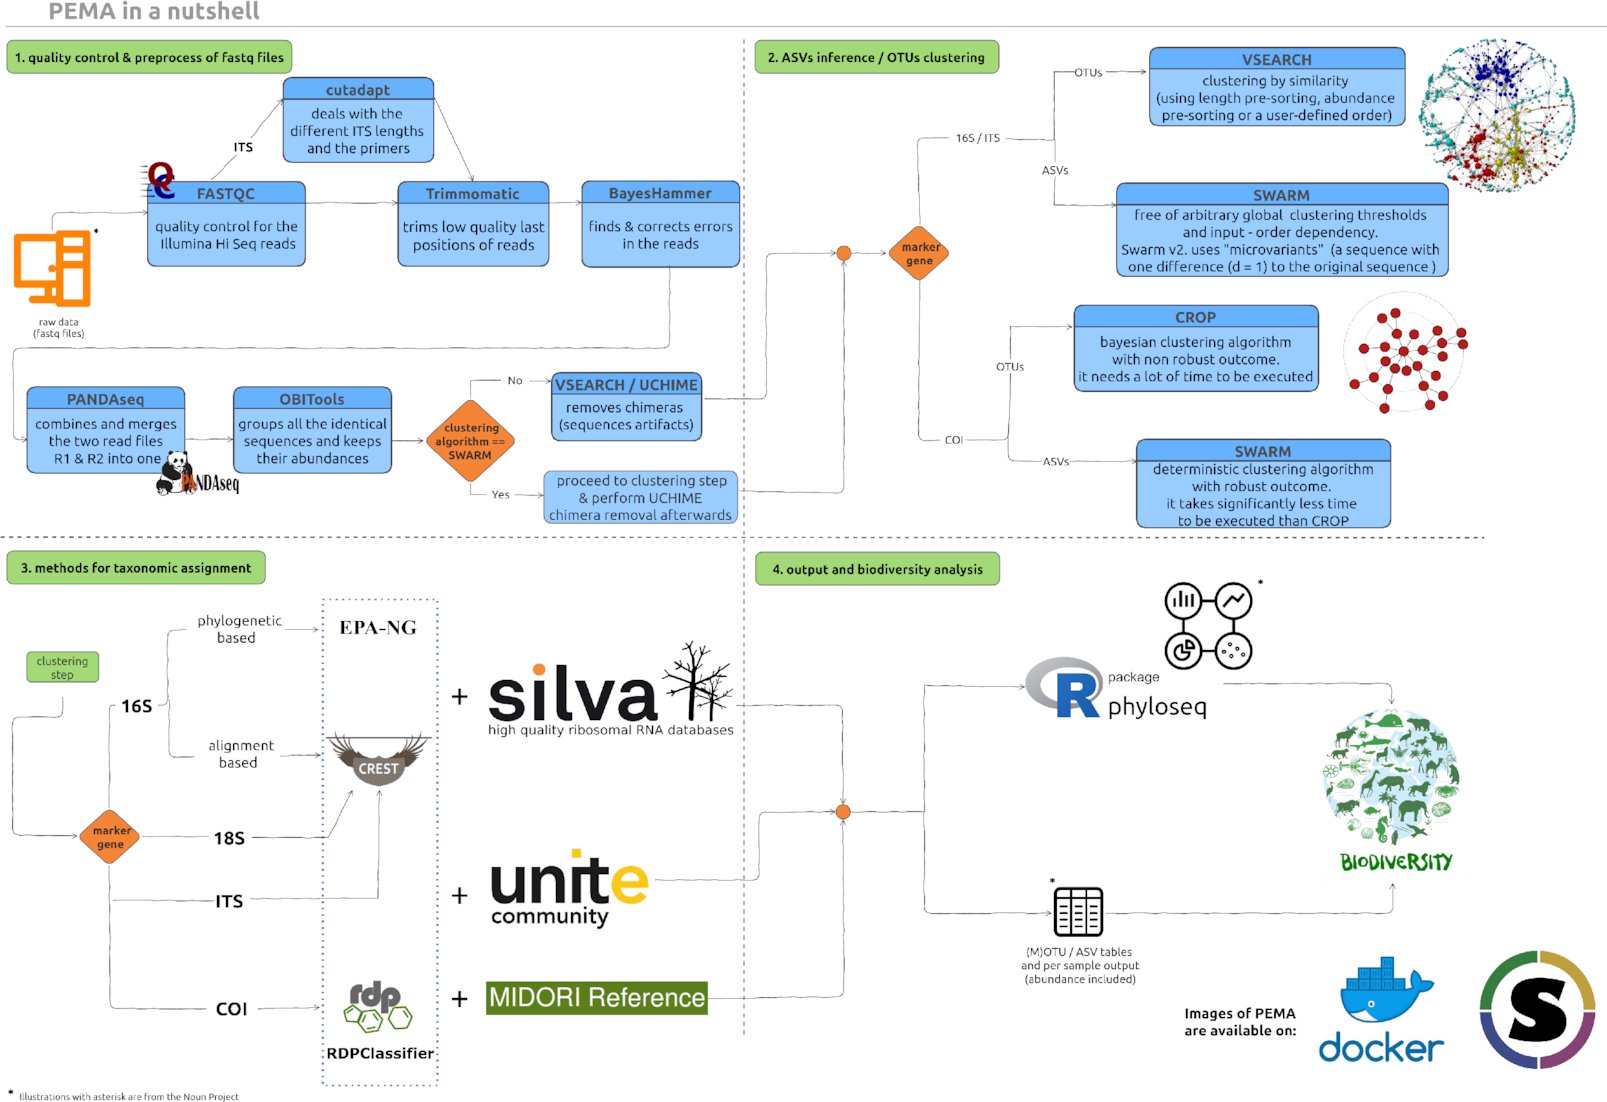
\includegraphics[width=0.95\columnwidth]{figures/pema_workflow.jpeg}
         \caption{The PEMA workflow: figure from publication}
      \end{figure}


   % PEMA CONTRIBUTION
   \subsection{Contribution}


   % PEMA METHODS
   \subsection{Methods \& Implementation}

   % PEMA RESULTS
   \subsection{Results \& Validation}


   % PEMA DISCUSSION
   \subsection{Discussion}



\newpage



% ----------------------------------------
% 
%      DARN
% 
% ----------------------------------------



% SECTION 3
\section[The Dark mAtteR iNvestigator (DARN) tool: getting to know the known unknowns in COI amplicon data]{The Dark mAtteR iNvestigator (DARN) tool: getting to know the known unknowns in COI amplicon data\footnote{For author contributions, please refer to the relevant section. Modified version of the published review.}}

\textbf{Citation:} \\
Zafeiropoulos, H., Gargan, L., Hintikka, S., Pavloudi, C. and Carlsson, J., 2021. The Dark mAtteR iNvestigator (DARN) tool: getting to know the known unknowns in COI amplicon data. Metabarcoding and Metagenomics, 5, p.e69657, \\
doi: \href{https://doi.org/10.3897/mbmg.5.69657}{10.3897/mbmg.5.69657}

\subsection{Introduction}

   % Parts of the following need to be moved in the main Intro


   In the case of eukaryotes, the target is most commonly mitochondrial due to higher copy numbers than nuclear DNA and the potential for species level identification. 
   Furthermore, mitochondria are nearly universally present in eukaryotic organisms, especially in case of metazoa, and can be easily sequenced and used for identification of the species composition of a sample \citep{taberlet2012towards}. 
   However, it is essential that comprehensive public databases containing well curated, up-to-date sequences from voucher specimens are available \citep{schenekar2020reference}. 
   This way, sequences generated by universal primers can be compared with the ones in reference databases, assessing sample OTU composition. 
   The taxonomy assignment step of the eDNA metabarcoding method and thus, the identification via DNA-barcoding, is only as good and accurate as the reference databases \citep{cilleros2019unlocking}. 
   Nevertheless, there is not a truly “universal” genetic marker that is capable of being amplified for all species across different taxa \citep{kress2015dna}. 
   Different markers have been used for different taxonomic groups \citep{deiner2017environmental}. 
   While bacterial and archaeal diversity is often based on the 16S rRNA gene, for eukaryotes a diverse set of loci is used from the analogous eukaryotic rRNA gene array (e.g., ITS, 18S or 28S rRNA), chloroplast genes (for plants) and mitochondrial DNA (for eukaryotes) in an attempt for species - specific resolution \citep{coissac2012bioinformatic}. 
   The mitochondrial cytochrome c oxidase subunit I (COI) marker gene has been widely used for the barcoding of the Animalia kingdom for almost two decades \citep{hebert2003barcoding}.
   There are cases where COI has been the standard marker for metabarcoding, such as in the assessment of freshwater macroinvertebrates \citep{elbrecht2017validation} even though not all taxonomic groups can be differentiated to the species level using this locus \citep{deiner2017environmental}; 
   for example, in case of fish other loci are widely used such as 12S rRNA gene (hereafter referred to as 12S rRNA) \citep{miya2020mifish}.


   The mitochondrial cytochrome c oxidase subunit I (also called cox1 or/and COI) is a gene fragment of ~700 bp, widely used for metazoan diversity assessment. Here we present some of the reasons that microbial eukaryotes and prokaryotes are also amplified in such studies, raising the issue of the known unknown sequences.

   COI is a fundamental part of the heme aa3-type mitochondrial cytochrome c oxidase complex: the terminal electron acceptor in the respiratory chain. 
   Even if aa3-type Cox have been found in bacteria, there are also other cytochrome c oxidase (Cox) groups, such as the cbb3-type cytochrome c oxidases (cbb3-Cox) and the cytochrome ba3 \citep{ekici2012biogenesis, schimo2017cytochrome}.

   Furthermore, the presence of highly divergent nuclear mitochondrial pseudogenes (numts) has been a widely known issue on the use of COI in barcoding and metabarcoding studies, leading to overestimates of the number of taxa present in a sample \citep{song2008many}.
   Numts are nonfunctional copies of mtDNA in the nucleus that have been found in major clades of eukaryotic organisms \citep{bensasson2001mitochondrial}.

   Thus, as Mioduchowska et al. (2018) \citep{mioduchowska2018instances} highlight, when universal primers are used targeting the COI locus, it is possible to co-amplify both non-target numts and prokaryotes \citep{siddall2009barcoding}. This has led to multiple erroneous DNA barcoding cases and it is now not rare to encounter bacterial sequences described as metazoan in databases such as GenBank \citep{mioduchowska2018instances}.



   Even though there are various known issues \citep{deagle2014dna}, COI is indeed considered as the “gold standard” for community DNA metabarcoding of bulk metazoan samples \citep{andujar2018coi}; 
   bulk is an environmental sample containing mainly organisms from the taxonomic group under study providing high quality and quantity of DNA \citep{taberletanalysis}. 
   However, as highlighted in the same study, this is not the case for eDNA samples. 
   As Stat et al. (2017) \citep{stat2017ecosystem} state, in the case of eDNA samples, the target region for metazoa is found in general at considerably lower concentrations compared to those from prokaryotes because most primers targeting the COI region amplify large proportions of prokaryotes at the same time \citep{yang2013testing, yang2014using, collins2019non}. 
   Cold-adapted marine gammaproteobacteria are an indicative example for this case as shown by Siddall et al. (2009) \citep{siddall2009barcoding}.



% DARN CONTRIBUTION
\subsection{Contribution}
   The co-amplification of prokaryotes explained above, is a major reason for why many Operational Taxonomic Units (OTUs) and/or Amplicon Sequence Variants (ASVs) in eDNA metabarcoding studies cannot get taxonomy assignments when metazoan reference databases are used (c.f. Aylagas et al. 2016 \citep{aylagas2016benchmarking}) or they are assigned to metazoan taxa but with very low confidence estimates. 
   Despite the presence of such OTUs/ASVs to a varying degree in metabarcoding studies using the COI marker gene \citep{siddall2009barcoding}, to the best of our knowledge, there has not been a thorough investigation of the origin for these sequences. 
   Although unassignable sequences could be informative, there have been few attempts to further investigate this dark matter (e.g., \citep{sinniger2016worldwide, haenel2017ngs}).
   The aim of this study was to build a framework for extracting such non-target, potentially unassigned (or assigned with low confidence) sequences from COI environmental sequence samples, hereafter referred to as “dark matter” as per Bernard et al. (2018) \citep{bernard2018microbial}. 
   We argue that the vast majority of these sequences represent microbial taxa, such as bacteria and archaea. 
   More specifically, based on the previously described methodology by Barbera et al. (2019) \citep{barbera2019epa} (see also full stack example of the EPA-ng algorithm) for large-scale phylogenetic placements, we built a framework to estimate to what extent the OTUs/ASVs retrieved in an environmental sample represent target taxa or not. 
   That is, to evaluate the taxonomy assignment step in a metabarcoding analysis, by checking the phylogenetic placement of dark matter sequences. Similar studies have provided great insight into other marker genes, e.g. \citep{jamy2020long}.


% DARN METHODS
\subsection{Methods \& Implementation}

\subsubsection*{Building the COI tree of life}

   Sequences for the COI region from all the three domains of life were retrieved from curated databases. 
   Eukaryotic sequences were retrieved from the Midori reference 2 database (version: GB239) \citep{machida2017metazoan}. 
   Initially, $1,315,378$ sequences were retrieved corresponding to $183,330$ unique species from all eukaryotic taxa. 
   With respect to bacteria and archaea, $3,917$ bacterial COI sequences were obtained from the BOLD database \citep{ratnasingham2007bold}. 
   Similarly, $117$ sequences from archaea were obtained from BOLD. 
   In addition, for all the PFam protein sequences related to the accession number for COX1 (\href{http://www.ncbi.nlm.nih.gov/nuccore/PF00115}{PF00115}), the respective DNA sequences were extracted from their corresponding genomes. 
   This way an additional $217$ archaeal and $9,154$ bacterial sequences were obtained (see Table 1). 
   In total, sequences from $15$ archaeal, $371$ bacterial families and 60 taxonomic groups of higher level not assigned in the family level, were gathered. 
   An overview of the approach that was followed is presented in Figure 1. 
   The large number of obtained sequences effectively prevents a phylogenetic tree construction encompassing their total number in terms of building a single phylogenetic tree covering all of the three domains of life (archaea, bacteria, eukaryota). 


   
   \begin{table}[h]
      \begin{tabular}{@{}lllll@{}}
      \toprule
      \multirow{2}{*}{\textbf{Resources}} & \multicolumn{2}{l}{\textbf{bacteria}} & \multicolumn{2}{l}{\textbf{archaea}} \\ \cmidrule(l){2-5} 
      & \textbf{\# of sequences} & \textbf{\# of strains} & \textbf{\# of sequences} & \textbf{\# of strains} \\ \cmidrule(r){1-1}
      BOLD & 3,917 & 2,267 & 117 & 117 \\
      PFam-oriented & 9,154 & 4,532 & 217 & 115 \\ \bottomrule
      \end{tabular}
      \caption{Number of sequences and taxonomic species per domain of life and resources. The (\#) symbols stands for "number".}
   \end{table}


   Therefore, consensus representative sequences from each of the three datasets were constructed using the PhAT algorithm (Czech et al. 2019); 
   based on the entropy of a set of sequences, PhAT groups sequences into a given target number of groups so they reflect the diversity of all the sequences in the dataset. 
   As PhAT uses a multiple sequence alignment (MSA) as input, all the three domain-specific datasets were aligned using the MAFFT alignment software tool v7.453 (Katoh et al. 2002). 
   In the case of Eukaryotes, the alignment of the corresponding sequences would be impractically long because of their large number ($~183$K sequences). 
   To address this challenge, a two-step procedure was followed; 
   a sequence subset of $500$ sequences (reference set) was selected and aligned and then used as a backbone for the alignment of all the remaining eukaryotic COI sequences. 
   All sequences were considered reliable as they were retrieved from curated databases (Midori2 and BOLD). 
   To build the reference set, a number ($n$) of the longest sequences from each of the various phyla were chosen, proportionally to the number ($m$) of sequences of each phylum (see Supplementary Table 1). 
   The --min-tax-level parameter of the PhAT algorithm corresponded to the class level, for the case of eukaryotes and to the family level for archaea and bacteria. 
   This parameter forced the PhAT algorithm to build at least one consensus sequence for each class and family respectively. 
   The taxonomy level was not the same for the case of eukaryotes sequence dataset and those of bacteria and archaea, as the number of unique eukaryotic families was one order of magnitude higher. 
   The PhAT algorithm was invoked through the gappa v0.6.1 collection of algorithms (Czech et al. 2020).








   \begin{figure}[h]
      \centering
      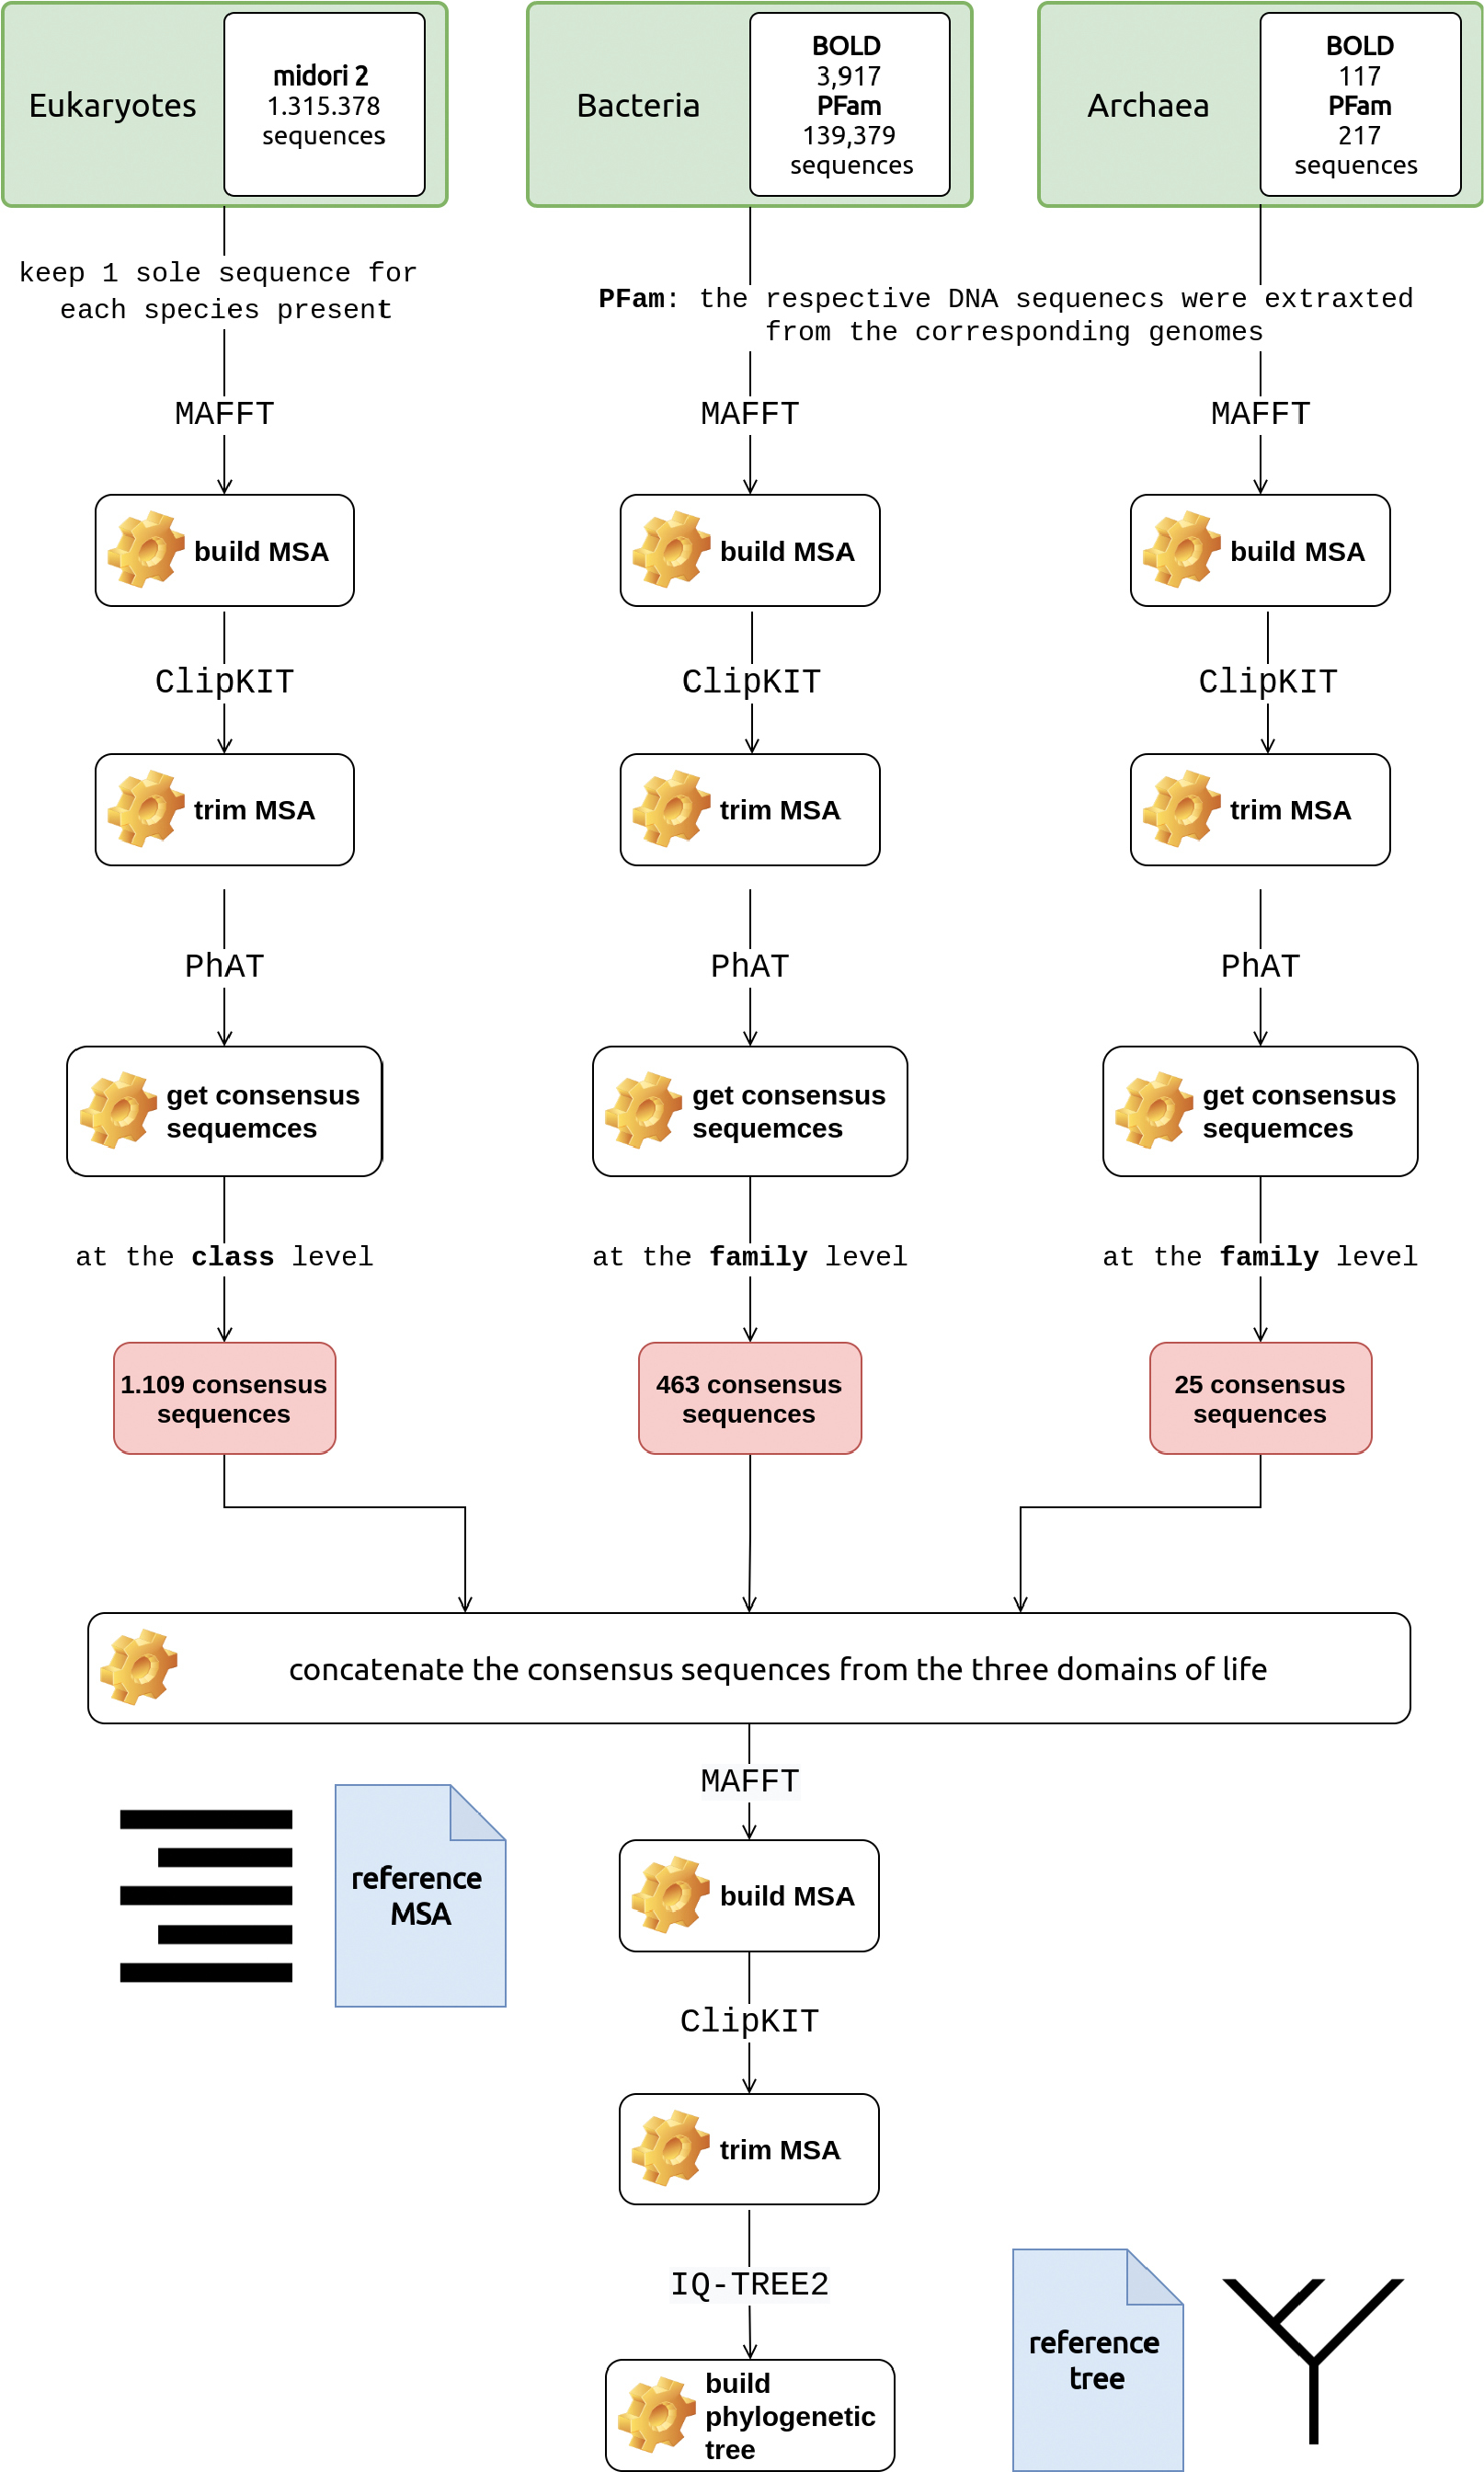
\includegraphics[width=100mm]{figures/darn_methodology.jpg}
      \caption{DARN methodology: figure in the publication}
   \end{figure}



% DARN RESULTS
\subsection{Results \& Validation}



\newpage

\begin{sidewaystable}
   
   \begin{tabular}{@{}ccccccccccc@{}}
   
   \toprule
   \thisfloatpagestyle{empty}
   \multirow{2}{*}{\begin{tabular}[c]{@{}c@{}}Sample(s) \\ accession number\end{tabular}} & \multirow{2}{*}{Envo type} & \multirow{2}{*}{Sample type} & \multirow{2}{*}{Primer set} & \multirow{2}{*}{\begin{tabular}[c]{@{}c@{}}Amplicon \\ length (bp)\end{tabular}} & \multirow{2}{*}{\begin{tabular}[c]{@{}c@{}}Bioinfo \\ pipeline(s)\end{tabular}} & \multirow{2}{*}{\# of ASVs} & \multicolumn{4}{c}{\begin{tabular}[c]{@{}c@{}}$\sim$\% of sequence assignments per domain \\ (if PEMA, using d = 10)\end{tabular}} \\ \cmidrule(l){8-11} 
    &  &  &  &  &  &  & \multicolumn{1}{c|}{Eukaryotes} & \multicolumn{1}{c|}{Bacteria} & \multicolumn{1}{c|}{Archaea} & \multicolumn{1}{c|}{distant} \\ \midrule
   \multirow{2}{*}{\begin{tabular}[c]{@{}c@{}}ERS6449795–\\ ERS6449829\end{tabular}} & \multirow{2}{*}{marine} & \multirow{2}{*}{eDNA} & \multirow{2}{*}{\begin{tabular}[c]{@{}c@{}}jgHCO2198 - \\ jgLCO1490 \\ and \\ LoboF1 - \\ LoboR1\end{tabular}} & \multirow{2}{*}{658} & \begin{tabular}[c]{@{}c@{}}QIIME2 - \\ Dada2\end{tabular} & 13,376 & 11 & 88.0 & 0.02 & 0.003 \\
    &  &  &  &  & \begin{tabular}[c]{@{}c@{}}PEMA \\ (d = 10)\end{tabular} & 39,454 & 25 & 75.0 & 0.1 & 0.4 \\
   \multirow{6}{*}{\begin{tabular}[c]{@{}c@{}}ERS6463899–\\ ERS6463901\end{tabular}} & \multirow{9}{*}{\begin{tabular}[c]{@{}c@{}}marine \\ reef\end{tabular}} & \multirow{15}{*}{eDNA} & \multirow{15}{*}{\begin{tabular}[c]{@{}c@{}}mlCOIintF - \\ jgHCO2198\end{tabular}} & \multirow{15}{*}{313} & JAMP & \multirow{5}{*}{1,304} & \multirow{5}{*}{35} & \multirow{5}{*}{65.0} & \multirow{5}{*}{-} & \multirow{5}{*}{0.2} \\
    &  &  &  &  & dada2 &  &  &  &  &  \\
    &  &  &  &  & PEAR &  &  &  &  &  \\
    &  &  &  &  & vsearch &  &  &  &  &  \\
    &  &  &  &  & DnoisE &  &  &  &  &  \\
    &  &  &  &  & \multirow{4}{*}{\begin{tabular}[c]{@{}c@{}}PEMA \\ (d = 10)\end{tabular}} & \multirow{4}{*}{11,545} & \multirow{4}{*}{46} & \multirow{4}{*}{50.0} & \multirow{4}{*}{1} & \multirow{4}{*}{3} \\
   \begin{tabular}[c]{@{}c@{}}ERS6463906–\\ ERS6463911\end{tabular} &  &  &  &  &  &  &  &  &  &  \\
   \begin{tabular}[c]{@{}c@{}}ERS6463913–\\ ERS6463918\end{tabular} &  &  &  &  &  &  &  &  &  &  \\
   \begin{tabular}[c]{@{}c@{}}ERS6463920–\\ ERS6463922\end{tabular} &  &  &  &  &  &  &  &  &  &  \\
   \multirow{6}{*}{\begin{tabular}[c]{@{}c@{}}ERS6463744–\\ ERS6463761\end{tabular}} & \multirow{6}{*}{\begin{tabular}[c]{@{}c@{}}marine \\ mangrove\end{tabular}} &  &  &  & JAMP & \multirow{5}{*}{663} & \multirow{5}{*}{40} & \multirow{5}{*}{60.0} & \multirow{5}{*}{-} & \multirow{5}{*}{0.6} \\
    &  &  &  &  & dada2 &  &  &  &  &  \\
    &  &  &  &  & PEAR &  &  &  &  &  \\
    &  &  &  &  & vsearch &  &  &  &  &  \\
    &  &  &  &  & DnoisE &  &  &  &  &  \\
    &  &  &  &  & \begin{tabular}[c]{@{}c@{}}PEMA \\ (d = 10)\end{tabular} & 5,879 & 49 & 47.0 & 1.0 & 2.0 \\
   ERR3460466 & marine & bulk & \multirow{3}{*}{\begin{tabular}[c]{@{}c@{}}mlCOIintF - \\ jgHCO2198\end{tabular}} & \multirow{3}{*}{313} & \multirow{3}{*}{\begin{tabular}[c]{@{}c@{}}PEMA \\ (d = 2)\end{tabular}} & 193 & 99 & 1 & - & - \\
   ERR3460467 & marine & bulk &  &  &  & 74 & 97 & 0.0 & - & 3 \\
   ERR3460470 & marine & eDNA &  &  &  & 184 & 71 & 28.0 & 0 & 1 \\
   ERS6488992 & lentic & \multirow{3}{*}{eDNA} & \multirow{3}{*}{\begin{tabular}[c]{@{}c@{}}fwhF2 - \\ EPTDr2\end{tabular}} & \multirow{3}{*}{142} & \multirow{3}{*}{\begin{tabular}[c]{@{}c@{}}PEMA \\ (d = 10)\end{tabular}} & 416 & 85 & 7 & 3 & 5 \\
   ERS6488993 & lentic &  &  &  &  & 315 & 99.2 & 0.4 & 0.4 & - \\
   ERS6488994 & lentic &  &  &  &  & 823 & 90 & 4 & 2 & 4 \\
   ERS6488995 & lotic & eDNA & BF3 - BR2 & 458 & \begin{tabular}[c]{@{}c@{}}PEMA \\ (d = 10)\end{tabular} & 1,940 & 64 & 34.0 & 2 & 0.3 \\ \bottomrule
   \end{tabular}

   \caption{DARN outcome over the samples or set of samples. Assignment fractions of the sequences per domain per sample in the DARN results over the samples.}

   
\end{sidewaystable}




% DARN DISCUSSION
\subsection{Discussion}

   By making use of a COI - oriented reference phylogenetic tree built from $1,593$ consensus sequences, to phylogenetically place sequences from COI metabarcoding samples onto it, the surmise for including bacteria, algae, fungi etc. \citep{yang2013testing, aylagas2016benchmarking} was verified. 
   Our results demonstrate that standard metabarcoding approaches based on the COI gene region of the mitochondrial genome will not only amplify eukaryotes, but also a large proportion of non-target prokaryotic organisms, such as bacteria and archaea. 
   Clearly, dark matter, and especially bacteria, make up a significant proportion of sequences generated in COI based eDNA metabarcoding datasets. 
   The large proportion of prokaryotes observed in the present study is corroborated by the findings of \citep{yang2013testing}. 
   Furthermore, dark matter seems to be particularly common in eDNA as compared to bulk samples \citep{andujar2018coi}. 
   However, it should be mentioned that the high number of prokaryotic sequences in COI metabarcoding data is also reflecting known issues with contamination 
   \citep{kumar2013blobology, dittami2017detection, de2020contaminations}, 
   incorrectly labeled reference sequences \citep{steinegger2020terminating} and holobionts 
   \citep{gilbert2012symbiotic, salvucci2016microbiome} in eukaryotic genomes.

   As publicly available bacterial COI sequences are far too few to represent the bacterial and archaeal diversity, their reliable taxonomic identification is not currently possible. 
   This way, bacterial, i.e. non-target, sequences that were amplified during the library preparation have at least the possibility of a taxonomy assignment. 
   Our implementations using DARN indicate that it is essential both for global reference databases (e.g., BOLD, Midori etc) and custom reference databases which are commonly used, to also include non-eukaryotic sequences.

   While our approach specifically addressed the COI gene, DARN can be adapted to analyse any locus fragment. 
   For instance, metabarcoding of environmental samples for the 12S rRNA mitochondrial region is often employed to assess fish biodiversity \citep{weigand2019dna, miya2020mifish} and the approach presented here could be adjusted to allow further analyses of the 12S rRNA data. 
   In addition, our approach can be used to identify non-target eukaryotes when the target is bacterial taxa \citep{huys2008coamplification}.

   The approaches implemented in DARN can benefit both bulk and eDNA metabarcoding studies, by allowing quality control and further investigation of the unassigned OTUs/ASVs. 
   The approach is also adaptable to other markers than COI. Moreover, the approach presented here allows researchers to better understand the known unknowns and shed light on the dark matter of their metabarcoding sequence data.



% % Table with COI and COI like sequences per rersource per domain
% \begin{table}[!htbp]
%    \begin{tabular}{lllll}
%    \hline
%    \multicolumn{1}{|l|}{\multirow{2}{*}{Resources}} & \multicolumn{2}{l|}{bacteria}                                             & \multicolumn{2}{l|}{archaea}                                              \\ \cline{2-5} 
%    \multicolumn{1}{|l|}{}                           & \multicolumn{1}{l|}{\# of sequences} & \multicolumn{1}{l|}{\# of strains} & \multicolumn{1}{l|}{\# of sequences} & \multicolumn{1}{l|}{\# of strains} \\ \hline
%    BOLD                                             & 3,917                                & 2,267                              & 117                                  & 117                                \\
%    PFam-oriented                                    & 9,154                                & 4,532                              & 217                                  & 115                                \\ \hline
%    \multicolumn{1}{|l|}{Total unique entries}       & \multicolumn{1}{l|}{11,421}          & \multicolumn{1}{l|}{6,798}         & \multicolumn{1}{l|}{334}             & \multicolumn{1}{l|}{201}           \\ \hline
%    \end{tabular}
%    \caption{Number of sequences and taxonomic species per domain of life and resources. The (\#) symbols stands for “number”.}
%    \label{tab:sequences_per_domain}
% \end{table}





% Phylogenetic tree figure with the placelemnts of the consensus seqs on the tree
% \begin{figure}[!htbp]
%    \centering
%    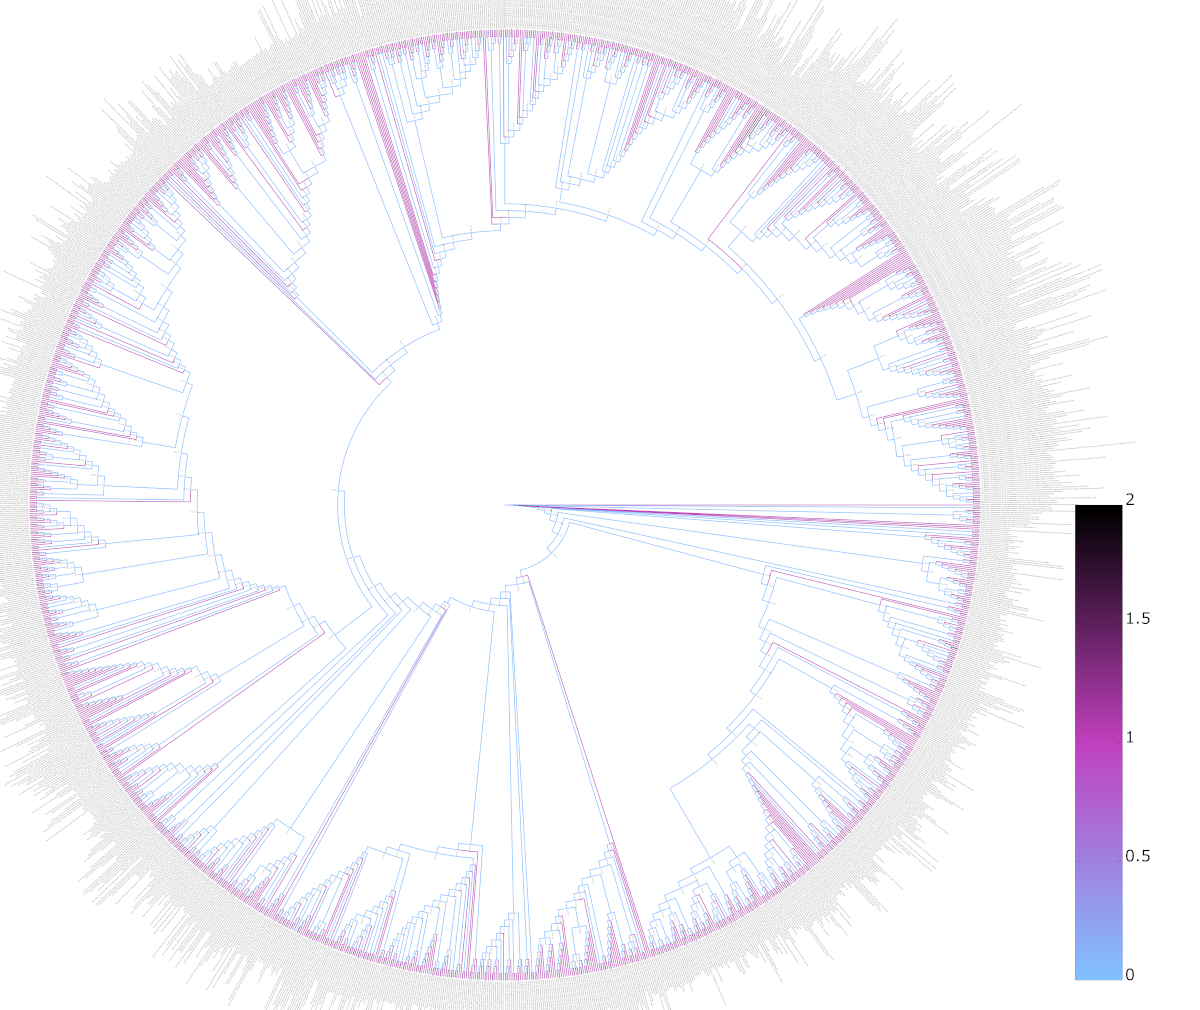
\includegraphics[width=0.65\columnwidth]{figures/darn_placemnets.png}
%    \caption{Placements of the consensus sequences used to build the COI reference phylogenetic tree for the DARN tool, onto the phylogenetic tree (stroke width for the branches of the tree is 5). The color coding represents the placements per branch, with a range from zero (blue) to a maximum of 2 (blue). The 1 leaf – 1 placement relationship, as well as the maximum of 2 placements in the color coding bar, indicate the proper placement of each consensus sequence to its corresponding branch.}
% \end{figure}


\section{A workflow for marine Genomic Observatories data analysis}






%%% Local Variables: 
%%% mode: latex
%%% TeX-master: "thesis"
%%% End: 
